\item \textbf{{[}IJC/PRELIM/9597/2018/P2/Q1{]} }

The Singapore Armed Forces is made up of many men and women who are
committed to protect the nation\textquoteright s peace and security.
The Ministry of Defence (MINDEF) keeps detailed personnel records
of all servicemen and servicewomen in a large database housed in the
central server at MINDEF Headquarters. Personnel records include career
history, salary, military rank, health details, achievements and awards.

The Human Resource Unit (HR) of MINDEF manages these records regularly
through a computerised system. Updates of the personnel\textquoteright s
records must be done within three working days once HR receives the
information from any military unit in MINDEF. Subsequently, administrative
officers of the military units in MINDEF will be able to view these
records via the intranet.

The current system has been used for the last fifteen years. MINDEF
wishes to replace this system with a new computerised system with
enhanced features and a better user interface. A system developer
is employed to carry out the task. 

MINDEF has accepted the proposal by the system developer, who will
address the following problems with the current system: 

\noindent %
\noindent\begin{minipage}[t]{1\columnwidth}%
\begin{enumerate}
\item[1.]  Poor database design 
\item[2.]  Limited types of reports that can be generated 
\item[3.]  Lack of intuitiveness of the user interface
\item[4.]  Slow system response time 
\item[5.]  Incompatibility with the current devices\textquoteright{} operating
systems
\item[6.]  Minimal security protection
\end{enumerate}
%
\end{minipage}
\begin{enumerate}
\item The system developer produces the following Program Evaluation and
Review Technique (PERT) chart:

A. Analysis of the solution 

B. Design of the solution 

C. Development of the solution

D. Documentation of the solution 

E. Implementation of the solution

F. Testing of the solution

Time is measured in weeks. \quad{} 
\begin{center}
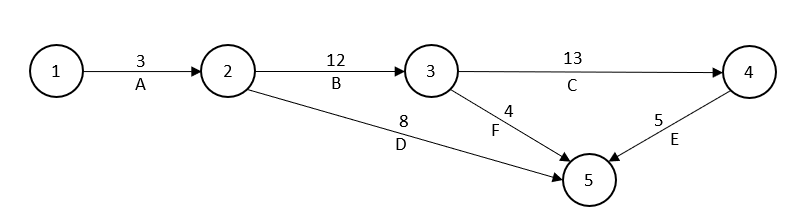
\includegraphics[width=0.5\paperwidth]{C:/Users/Admin/Desktop/Github/question_bank/LyX/static/img/9597-IJC-2018-P2-Q1-1}
\par\end{center}

From the PERT chart, 
\begin{enumerate}
\item state the critical path.\hfill{} {[}1{]}
\item state the minimum time in which the project can be completed. \hfill{}{[}1{]}
\item describe and give an example of concurrent activities. \hfill{}{[}2{]}
\item describe and give an example of dependent activities.\hfill{} {[}2{]}
\end{enumerate}
\item The system developer is required to provide more details in the PERT
chart. It is proposed that Activity F should be removed from the chart
and three new activities added:

J. Black box testing -- 2 weeks 

K. White box testing -- 2 weeks

L. Beta testing -- 3 weeks

Redraw the PERT chart to show the effects of these changes. \hfill{}{[}4{]}
\item Draw a sketch of the Gantt chart to show the information in \textbf{(a)}.
\hfill{}{[}6{]}
\item Maintenance will be required after implementing the new system.

Describe two types of maintenance. For each type, give an example
for this new system. \hfill{}{[}6{]}
\item The new system will provide all staff in HR with full access to all
personnel records. The administrative officers of the military unit
will have only read access to the data. Only designated computers
in the MINDEF network are able to access the system.

Describe \textbf{three} ways in which the security of this system
can be maintained. \hfill{}{[}6{]}
\item MINDEF is considering to allow servicemen and servicewomen to update
their own personnel records directly into the system via the internet.
Describe one security concern and one ethical issue that may arise
due to this proposed implementation.\hfill{} {[}2{]}
\end{enumerate}